\section{Prezentacja wyników pracy}
    Do dnia 27.04.2023r. wykonano następujące zadania:
    \begin{itemize}
        \item zaprojektowano układ czujników,
        \item opracowano transmisje danych z mikrokontrolera do komputera,
        \item określono sumę kontrolną dla opracowanej transmisji danych,
        \item zaprojektowano grafikę aplikacji,
        \item zaimplementowano zakładkę ,,wszystkie parametry''. 
    \end{itemize}

    \subsection{Protokół komunikacji}
        Komunikacja odbywa się poprzez UART. Ramka składa się z 13 bajtów. Dane 
        zbierane z czujników mogą okazać się większe niż 1 bajt wiec,
        przed wysłaniem dzielone są na 2 części i wysyłane jako 1 bajtowe. Program odbierający
        skleja je ze sobą do postaci 2 bajtowej. Dane wysyłane są w postaci  binarnej,
        w następujący sposób:
        \begin{itemize}
            \item Bajt 1: START -> 0xFF
            \item Bajt 2: OBJĘTOŚĆ -> 8 najstarszych bitów
            \item Bajt 3: OBJĘTOŚĆ -> 8 najmłodszych bitów
            \item Bajt 4: TEMPERATURA\_1 -> 8 najstarszych bitów
            \item Bajt 5: TEMPERATURA\_1 -> 8 najmłodszych  bitów
            \item Bajt 6: TEMPERATURA\_2 -> 8 najstarszych bitów
            \item Bajt 7: TEMPERATURA\_2 -> 8 najmłodszych  bitów
            \item Bajt 8: WILGOTNOŚĆ\_1 ->  8 najstarszych bitów
            \item Bajt 9: WILGOTNOŚĆ\_1 ->  8 najmłodszych bitów
            \item Bajt 10: WILGOTNOŚĆ\_2 ->  8 najstarszych  bitów
            \item Bajt 11: WILGOTNOŚĆ\_2 ->  8 najmłodszych  bitów
            \item Bajt 12: SUMA KONTROLNA -> CRC8
            \item Bajt 13: STOP -> 0xFE
        \end{itemize}
    \subsection{Aplikacja}
        \begin{figure}[H]
            \centering
            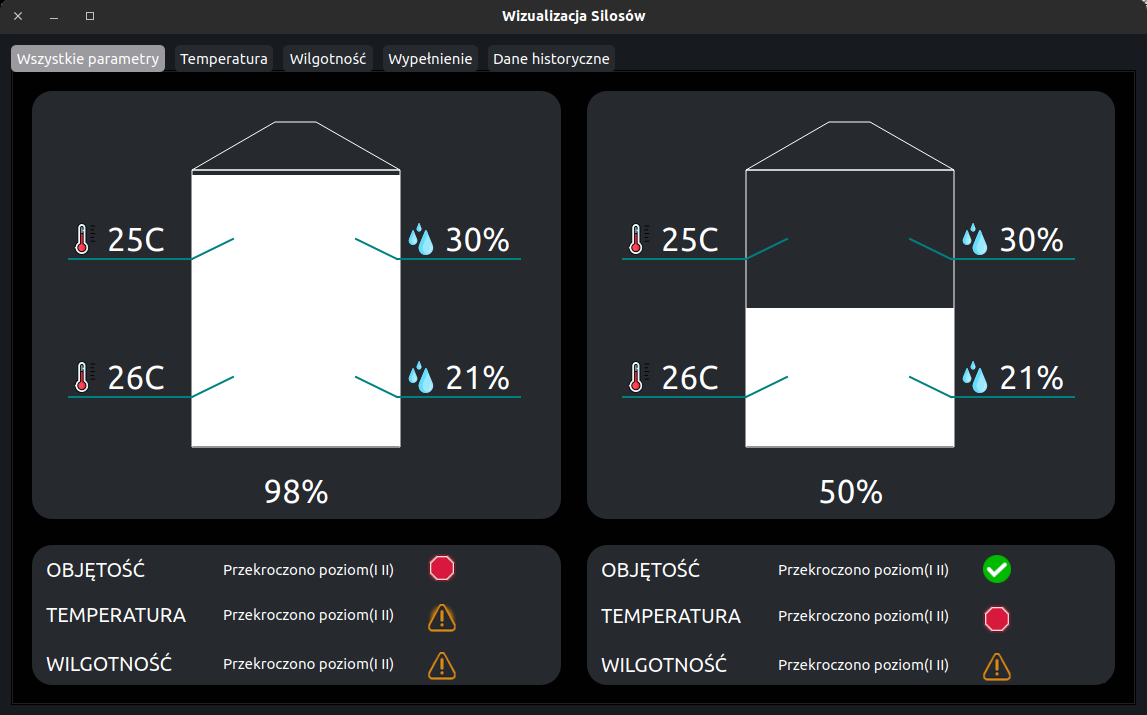
\includegraphics[width = \textwidth]{obrazy/zakladka_wszystkie_parametry.png}
            \caption{Wygląd zakładki wszystkie parametry}
        \end{figure}

        Ui zostało zaprojektowane za pomocą narzędzia Designer. Rysowanie silosów, ich wypełnienia i pozostałych 
        informacji zostało zrealizowane za pomocą reimplementacji metody painEvent. 
        Kod został udokumentowany za pomocą programu doxygen.